\chapter{Modello dell'\textit{on-line} HDF}\label{ch:online}

Si immagini di costruire il modellino di un'abitazione, utilizzando quei mattoncini di plastica che i bambini usano solitamente per giocare. Per fare ciò è indispensabile possedere i mattoncini (in forme e dimensioni variabili), conoscere le regole per impilarli (ad esempio, diremo che un mattoncino è impilato correttamente ad un altro se risultano saldamente incastrati fra loro), e utilizzare la propria creatività per creare un modello di abitazione che sia il più vicino possibile a quella ideale che si vuole costruire. La costruzione di un modello matematico non è molto diverso dal gioco delle costruzioni. I mattoncini sono le relazioni costitutive illustrate nel capitolo precedente (si tratta di equazioni fisico-empiriche a sè stanti e diverse fra loro), le regole per l'incastro dei mattoncini sono le leggi generali di conservazione (massa, volume, \ldots), e in questo capitolo verrà mostrato come, conoscendo a grandi linee come funziona l'organismo umano e la macchina dializzatrice e come questi due apparati sono connessi (\figurename\ref{schema_generale}), con un po' di creatività e buon senso si riuscirà a costruire un modello matematico per l'emodiafiltrazione.
\begin{figure}[htbp]
	\centering
		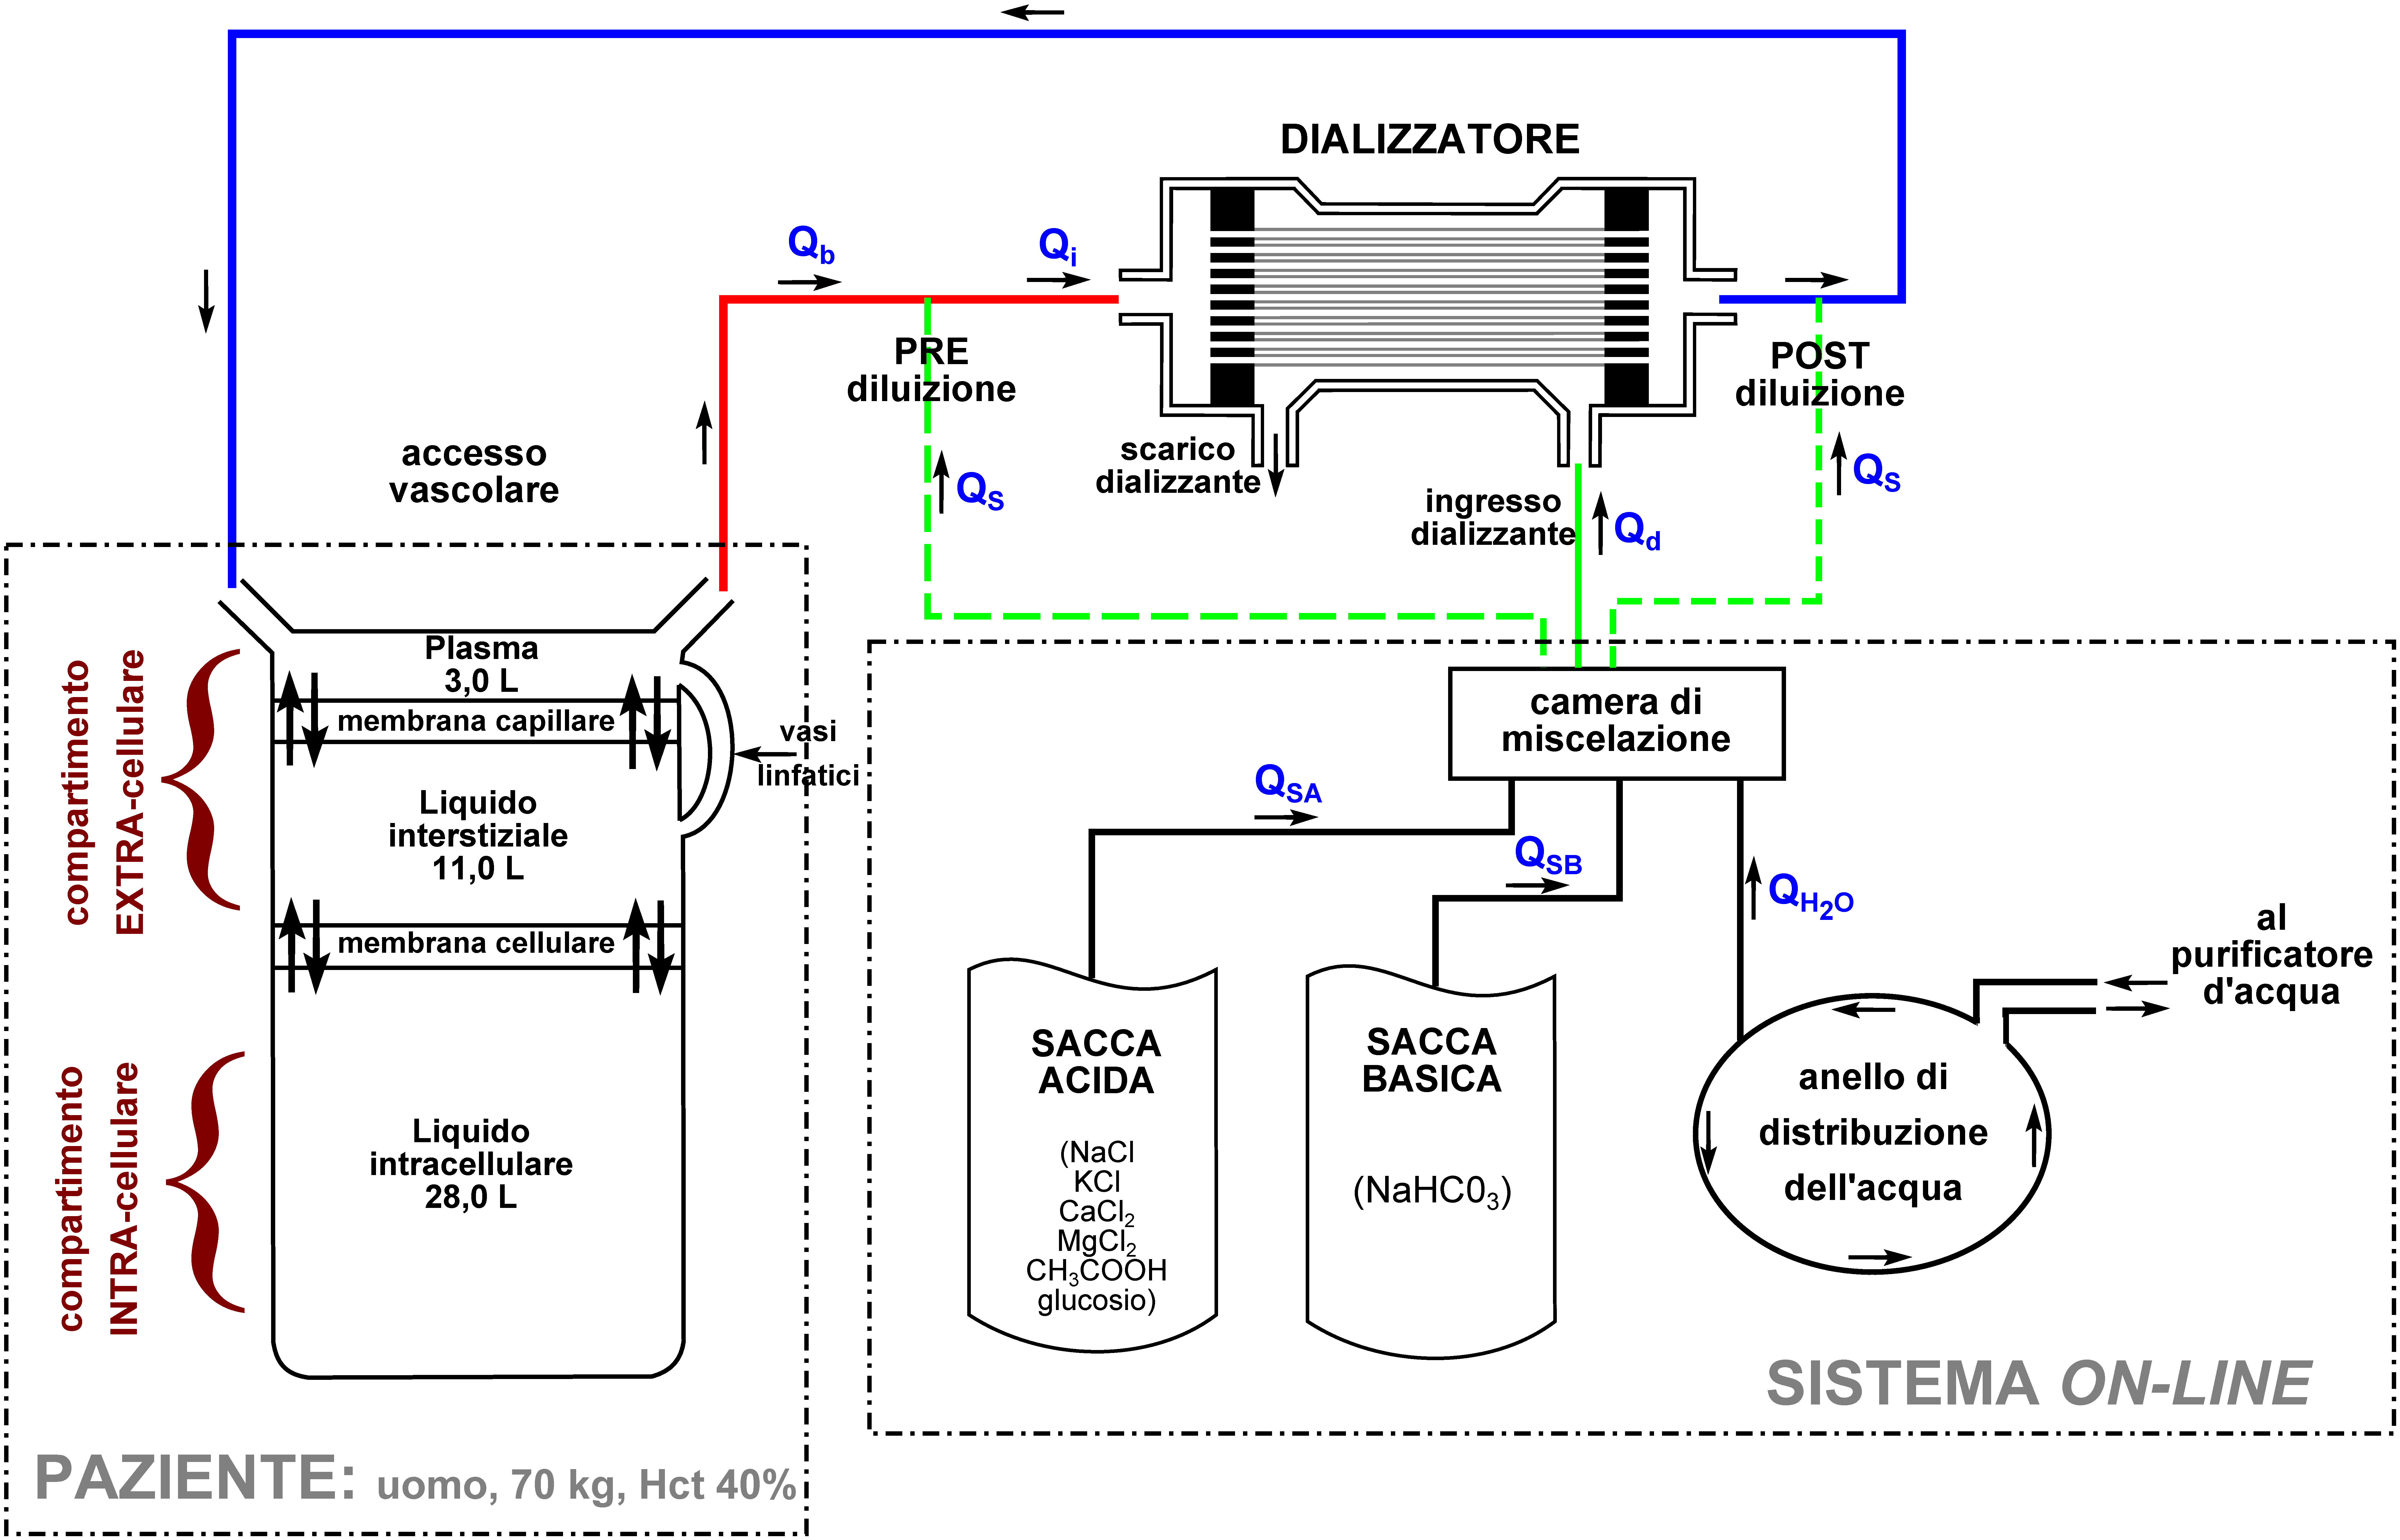
\includegraphics[width=\textwidth]{immagini/schema_generale.eps}
	\caption{Schema generale dell'\textit{on-line} HDF.}
	\label{schema_generale}
\end{figure}

\input capitoli/sections/sec_modello_online.tex
\input capitoli/sections/sec_modello_paziente.tex
\input capitoli/sections/sec_modello_inizializzazione.tex
\input capitoli/sections/sec_modello_implementazione.tex
\input capitoli/sections/sec_modello_scelta_parametri.tex